\documentclass[]{tufte-handout}

% ams
\usepackage{amssymb,amsmath}

\usepackage{ifxetex,ifluatex}
\usepackage{fixltx2e} % provides \textsubscript
\ifnum 0\ifxetex 1\fi\ifluatex 1\fi=0 % if pdftex
  \usepackage[T1]{fontenc}
  \usepackage[utf8]{inputenc}
\else % if luatex or xelatex
  \makeatletter
  \@ifpackageloaded{fontspec}{}{\usepackage{fontspec}}
  \makeatother
  \defaultfontfeatures{Ligatures=TeX,Scale=MatchLowercase}
  \makeatletter
  \@ifpackageloaded{soul}{
     \renewcommand\allcapsspacing[1]{{\addfontfeature{LetterSpace=15}#1}}
     \renewcommand\smallcapsspacing[1]{{\addfontfeature{LetterSpace=10}#1}}
   }{}
  \makeatother

\fi

% graphix
\usepackage{graphicx}
\setkeys{Gin}{width=\linewidth,totalheight=\textheight,keepaspectratio}

% booktabs
\usepackage{booktabs}

% url
\usepackage{url}

% hyperref
\usepackage{hyperref}

% units.
\usepackage{units}


\setcounter{secnumdepth}{-1}

% citations

% pandoc syntax highlighting
\usepackage{color}
\usepackage{fancyvrb}
\newcommand{\VerbBar}{|}
\newcommand{\VERB}{\Verb[commandchars=\\\{\}]}
\DefineVerbatimEnvironment{Highlighting}{Verbatim}{commandchars=\\\{\}}
% Add ',fontsize=\small' for more characters per line
\newenvironment{Shaded}{}{}
\newcommand{\AlertTok}[1]{\textcolor[rgb]{1.00,0.00,0.00}{\textbf{#1}}}
\newcommand{\AnnotationTok}[1]{\textcolor[rgb]{0.38,0.63,0.69}{\textbf{\textit{#1}}}}
\newcommand{\AttributeTok}[1]{\textcolor[rgb]{0.49,0.56,0.16}{#1}}
\newcommand{\BaseNTok}[1]{\textcolor[rgb]{0.25,0.63,0.44}{#1}}
\newcommand{\BuiltInTok}[1]{#1}
\newcommand{\CharTok}[1]{\textcolor[rgb]{0.25,0.44,0.63}{#1}}
\newcommand{\CommentTok}[1]{\textcolor[rgb]{0.38,0.63,0.69}{\textit{#1}}}
\newcommand{\CommentVarTok}[1]{\textcolor[rgb]{0.38,0.63,0.69}{\textbf{\textit{#1}}}}
\newcommand{\ConstantTok}[1]{\textcolor[rgb]{0.53,0.00,0.00}{#1}}
\newcommand{\ControlFlowTok}[1]{\textcolor[rgb]{0.00,0.44,0.13}{\textbf{#1}}}
\newcommand{\DataTypeTok}[1]{\textcolor[rgb]{0.56,0.13,0.00}{#1}}
\newcommand{\DecValTok}[1]{\textcolor[rgb]{0.25,0.63,0.44}{#1}}
\newcommand{\DocumentationTok}[1]{\textcolor[rgb]{0.73,0.13,0.13}{\textit{#1}}}
\newcommand{\ErrorTok}[1]{\textcolor[rgb]{1.00,0.00,0.00}{\textbf{#1}}}
\newcommand{\ExtensionTok}[1]{#1}
\newcommand{\FloatTok}[1]{\textcolor[rgb]{0.25,0.63,0.44}{#1}}
\newcommand{\FunctionTok}[1]{\textcolor[rgb]{0.02,0.16,0.49}{#1}}
\newcommand{\ImportTok}[1]{#1}
\newcommand{\InformationTok}[1]{\textcolor[rgb]{0.38,0.63,0.69}{\textbf{\textit{#1}}}}
\newcommand{\KeywordTok}[1]{\textcolor[rgb]{0.00,0.44,0.13}{\textbf{#1}}}
\newcommand{\NormalTok}[1]{#1}
\newcommand{\OperatorTok}[1]{\textcolor[rgb]{0.40,0.40,0.40}{#1}}
\newcommand{\OtherTok}[1]{\textcolor[rgb]{0.00,0.44,0.13}{#1}}
\newcommand{\PreprocessorTok}[1]{\textcolor[rgb]{0.74,0.48,0.00}{#1}}
\newcommand{\RegionMarkerTok}[1]{#1}
\newcommand{\SpecialCharTok}[1]{\textcolor[rgb]{0.25,0.44,0.63}{#1}}
\newcommand{\SpecialStringTok}[1]{\textcolor[rgb]{0.73,0.40,0.53}{#1}}
\newcommand{\StringTok}[1]{\textcolor[rgb]{0.25,0.44,0.63}{#1}}
\newcommand{\VariableTok}[1]{\textcolor[rgb]{0.10,0.09,0.49}{#1}}
\newcommand{\VerbatimStringTok}[1]{\textcolor[rgb]{0.25,0.44,0.63}{#1}}
\newcommand{\WarningTok}[1]{\textcolor[rgb]{0.38,0.63,0.69}{\textbf{\textit{#1}}}}

% longtable

% multiplecol
\usepackage{multicol}

% strikeout
\usepackage[normalem]{ulem}

% morefloats
\usepackage{morefloats}


% tightlist macro required by pandoc >= 1.14
\providecommand{\tightlist}{%
  \setlength{\itemsep}{0pt}\setlength{\parskip}{0pt}}

% title / author / date
\title{A bayesian approach to identify mortgage default rate at city leve}
\author{Andres Potapczynski, Jongwoo Choi, Yi Chen}
\date{28 January 2018}


\begin{document}

\maketitle



{
\setcounter{tocdepth}{2}
\tableofcontents
}

\hypertarget{abstract}{%
\subsection*{Abstract}\label{abstract}}
\addcontentsline{toc}{subsection}{Abstract}

\hypertarget{data}{%
\section{Data}\label{data}}

\hypertarget{introduction}{%
\subsection{Introduction}\label{introduction}}

\hypertarget{explortary-data-analysis}{%
\subsection{Explortary Data Analysis}\label{explortary-data-analysis}}

\hypertarget{data-processin}{%
\subsection{Data Processin}\label{data-processin}}

The data in our model has been processed the following steps: * Take the
log of `client\_income' and `asset\_market\_value'.

Reason: The distribution of these two variables are highly right skewed
with high-value outliers. * Standardized the design matrix.

Reason: Improve the coverage of MCMC. Exclude intercept in the design
matrix. Reason: variables are centered and the ICR model has been used.

\hypertarget{baseline-model-linear-binormial-regression}{%
\section{Baseline Model : Linear Binormial
Regression}\label{baseline-model-linear-binormial-regression}}

\hypertarget{model-extension-car-zero-inflation}{%
\section{Model Extension: CAR \& Zero
Inflation}\label{model-extension-car-zero-inflation}}

\hypertarget{a-linear-binormial-regression-analogy}{%
\subsection{A linear binormial regression
analogy}\label{a-linear-binormial-regression-analogy}}

Lik what we did in the baseline model. We process by treating the
underlying deterministic model as providing an expected default times
for each city around which there will be variation due to both
measurement error and simplifications. Consider the typical formulation
of a linear regression, where \(y_n\) is the is an observable default
time, \(x_n\) is a row vector of unmodeled predictors ( independent
variables), \(\beta\) is a coefficient vector parameter and we separate
the intercep as \(a\). In the city level, we assume that the number of
individual records in city \(i\) is \(n_i\).Thus, we have the model:

\[ y_i \sim Binormial(n_{i},logit^{-1}(a + x_i\beta)) \] As a robust
prior distribution option, we take
\(\beta \sim cauchy(location=0,scale=2.5)\).

In model 2, we will extend this model in two ways: (1) incoperate the
geographic state information (2) zero inflated model.

\hypertarget{extension-one-incoperate-geographic-information}{%
\subsubsection{Extension one: Incoperate Geographic
Information}\label{extension-one-incoperate-geographic-information}}

In this project, we utilize the IAR prior for state feature. Intrisnic
conditional autoregressive (IAR) is an extension of conditional
autoregressive (CAR) models, which are popular as prior distributions
for spatial random effects with areal spatial data. In our model, we
have a random quantity \(\phi = (\phi_1,\phi_2,...,\phi_{32})\) at 32
state areal locations. In each state, we have the individual records
aggregated at the city level. And each city data belong to one state.
According to the Brook's Lemma, the joint the distribution of \(\phi\)
can be expressed as the followings:
\[\phi \sim N(0,[D_{\tau} (I-\alpha B)]^{-1})\] In this formula, we
have:

\begin{itemize}
\item
  \(D = diag(m_i)\) is an \(32 \times 32\) diagonal matrix with \(m_i\)
  is the number of the neighbors for the state i
\item
  \(D_{\tau} = \tau D\) and \(\tau\) is the hyperparameter in the
  conditional distributions of the \(\phi\)
\item
  \(\alpha\) is the parameter that controls spatial dependence. In IAR,
  we let \(\alpha =1\)
\item
  \(B = D^{-1} W\) is the scaled adjacency matrix. And \(W\) is the
  adjacency matrix. (\(w_{ii}=0\),\(w_{ij}=1\) if the state i is a
  neighbor of state j , and \(w_{ij}=1\) otherwise)
\end{itemize}

We can simplifies the IAR model to:

\[\phi \sim N(0,\tau (D-W)]^{-1})\] In IAR model, we have a singular
precision matrix and an improper prior distribution. However, in
practice, IAR models are fit with a sum to zero constrains:
\(\sum_{i}\phi_i = 0\) for each connected component of the graph. In
this way, we can interpret both overall means and the component-wise
means.

Through log probability accumulator, we can accure computational
efficiency gains. We have:

\[log(p(\phi | \tau)) = -\frac{n}{2}log(2\pi) + \frac{1}{2}log(det^{*}(\tau(D-W))) - \frac{1}{2}\phi^{T}\tau(D-W)\phi\]
\[=-\frac{n}{2}log(2\pi) + \frac{1}{2}log(\tau^{n-k}) + \frac{1}{2}log(det^{*}(\tau(D-W))  - \frac{1}{2}\phi^{T}\tau(D-W)\phi\]

In this formula, \(det^{*}(A)\) is the generlized determinant of the
square matrix A defined as the product of its non-zero eigenvalues, and
the k is the number of the connented component in the graph.(k=1 for our
data) Dropping the additive constants, the qunantity to increment
becomes:

\[  \frac{1}{2}log(\tau^{n-k}) - \frac{1}{2}\phi^{T}\tau(D-W)\phi \]

In our model, we assume the hyperparameter
\(\tau \sim Gamma(shape = 2,rate = 2)\). We define the sparse\_iar\_lpdf
function as a more efficient spare representation as the following:

\begin{Shaded}
\begin{Highlighting}[]
\NormalTok{functions \{}
\NormalTok{  real }\KeywordTok{sparse_iar_lpdf}\NormalTok{(vector phi, real tau, int[,] W_sparse, vector D_sparse, vector lambda, int S, int W_n) \{}
\NormalTok{      row_vector[S] phit_D; }\OperatorTok{/}\ErrorTok{/}\StringTok{ }\NormalTok{phi}\StringTok{' * D}
\StringTok{      row_vector[S] phit_W; // phi'} \OperatorTok{*}\StringTok{ }\NormalTok{W}
\NormalTok{      vector[S] ldet_terms;}
    
\NormalTok{      phit_D =}\StringTok{ }\NormalTok{(phi .}\OperatorTok{*}\StringTok{ }\NormalTok{D_sparse)}\StringTok{';}
\StringTok{      phit_W = rep_row_vector(0, S);}
\StringTok{      for (i in 1:W_n) \{}
\StringTok{        phit_W[W_sparse[i, 1]] = phit_W[W_sparse[i, 1]] + phi[W_sparse[i, 2]];}
\StringTok{        phit_W[W_sparse[i, 2]] = phit_W[W_sparse[i, 2]] + phi[W_sparse[i, 1]];}
\StringTok{      \}}
\StringTok{    }
\StringTok{      return 0.5 * ((S-1) * log(tau)}
\StringTok{                    - tau * (phit_D * phi - (phit_W * phi)));}
\StringTok{  \}}
\StringTok{\}}
\end{Highlighting}
\end{Shaded}

After we get the IAR prior, we can take it into our model.For the \(i\)
the city in the \(j\) the state, we have:

\[ y_{ij} \sim Binormial(n_{ij},logit^{-1}(a + \phi_j + x_{ij}\beta)) \]
* Reason for design the model in this way rather than hierarchical
model:

\begin{enumerate}
\def\labelenumi{\arabic{enumi}.}
\item
  Hierarchical extension will greatly expend the demension of the
  parameter space. Consequently, the estimation convergence would be
  much more difficult.Just focus on the binormial regression part. If we
  take the hierarchical extension both on the intercept and coefficient
  terms, there will have \(32 \times 1 = 32\) intercept paramters and
  \(32 \times 7 = 224\) coefficient parameters (total 256
  parameters).For taking the hierarchical extension on \(\beta\)s, we
  have 1 intercept and \(7 \times 32 = 224\) coefficient in the
  binormial regression model (total 225 parameters). But now, we only
  have 1 parameter for overall intercept, 32 parameter for the state
  level effecr and 7 parameter for the different independent variables'
  effects.
\item
  This design of model is better for interpreation and better for us to
  solve our research problems.Now the coefficient terms are not depend
  on the state prior. Thus, we can estimate the overall effect from
  these independent variables, like age and income. And on the state
  level effect, we can have the overall idea based on the estimated
  parameter values.
\end{enumerate}

\hypertarget{extension-two-zero-inflated-model}{%
\subsection{Extension two: zero inflated
model}\label{extension-two-zero-inflated-model}}

Zero-inflated model originally provide mixture of a mixtures of a
Poisson and Bernoulli probability mass function to allow more
flexibility in modeling the probability of a zero outcome. Zero-inflated
models, as defined by Lambert (1992), add additional probability mass to
the outcome of zero. But, this extension can also be applied for other
categorical distributions like binomial distribution we used in this
project.

We assume a parameter \(\theta\) as the probability of drawing a zero
and the probability \(1-\theta\) as drawing fro mthe Binormal
distribution. The prior distribution of \(\theta\) is uniform between 0
and 1, since we have no extra information about this parameter. The
distribution function is thus:

\[p(y_n | \theta,a,\beta) =\begin{cases} 
\theta + (1-\theta) \times Binomial(0 |a,\beta,\phi ) & y_n =0 \\
(1-\theta) \times Binomial(0 |a,\beta,\phi )  & y_n > 0 \end{cases}\]

In stan, we estimate the model in this following ways:

\begin{Shaded}
\begin{Highlighting}[]
\ControlFlowTok{for}\NormalTok{ (j }\ControlFlowTok{in} \DecValTok{1}\OperatorTok{:}\NormalTok{N_train)\{}
    \ControlFlowTok{if}\NormalTok{ (y[j] }\OperatorTok{==}\StringTok{ }\DecValTok{0}\NormalTok{)\{}
\NormalTok{      target }\OperatorTok{+}\ErrorTok{=}\StringTok{ }\KeywordTok{log_sum_exp}\NormalTok{(}\KeywordTok{bernoulli_lpmf}\NormalTok{(}\DecValTok{1} \OperatorTok{|}\StringTok{ }\NormalTok{theta), }\KeywordTok{bernoulli_lpmf}\NormalTok{(}\DecValTok{0} \OperatorTok{|}\StringTok{ }\NormalTok{theta) }\OperatorTok{+}\StringTok{ }\KeywordTok{binomial_logit_lpmf}\NormalTok{(y[j] }\OperatorTok{|}\StringTok{ }\NormalTok{n_city_train[j],alpha[state_train[j]] }\OperatorTok{+}\StringTok{ }\NormalTok{X_train[j,]}\OperatorTok{*}\StringTok{ }\NormalTok{beta));}
\NormalTok{      \}}
    \ControlFlowTok{else}\NormalTok{\{}
\NormalTok{      target }\OperatorTok{+}\ErrorTok{=}\StringTok{ }\KeywordTok{bernoulli_lpmf}\NormalTok{(}\DecValTok{0} \OperatorTok{|}\StringTok{ }\NormalTok{theta) }\OperatorTok{+}\StringTok{ }\KeywordTok{binomial_logit_lpmf}\NormalTok{(y[j] }\OperatorTok{|}\StringTok{ }\NormalTok{n_city_train[j],alpha }\OperatorTok{+}\StringTok{ }\NormalTok{X_train[j,] }\OperatorTok{*}\StringTok{ }\NormalTok{beta);\}}
\NormalTok{  \}}
\end{Highlighting}
\end{Shaded}

And we predict the \(y_{rep}\) in the following way:

\begin{Shaded}
\begin{Highlighting}[]
\NormalTok{generated quantities\{}
\NormalTok{  int y_rep[N_train];}
\NormalTok{  real}\OperatorTok{<}\NormalTok{lower =}\DecValTok{0}\NormalTok{,upper=}\DecValTok{1}\OperatorTok{>}\StringTok{ }\NormalTok{zero_train[N_train];}
  \ControlFlowTok{for}\NormalTok{ (i }\ControlFlowTok{in} \DecValTok{1}\OperatorTok{:}\NormalTok{N_train)\{}
\NormalTok{    zero_train[i] =}\StringTok{ }\KeywordTok{uniform_rng}\NormalTok{(}\DecValTok{0}\NormalTok{,}\DecValTok{1}\NormalTok{);}
    \ControlFlowTok{if}\NormalTok{ (zero_train[i] }\OperatorTok{<}\StringTok{ }\NormalTok{theta)\{}
\NormalTok{      y_rep[i] =}\StringTok{ }\DecValTok{0}\NormalTok{;}
\NormalTok{      \}}
    \ControlFlowTok{else}\NormalTok{\{}
\NormalTok{      y_rep[i] =}\StringTok{ }\KeywordTok{binomial_rng}\NormalTok{(n_city_train[i],}\KeywordTok{inv_logit}\NormalTok{(alpha[state_train[i]] }\OperatorTok{+}\StringTok{ }\NormalTok{X_train[i,]}\OperatorTok{*}\StringTok{ }\NormalTok{beta));}
\NormalTok{      \}}
\NormalTok{  \}}
\NormalTok{\}}
\end{Highlighting}
\end{Shaded}

\hypertarget{model-coveage-testing-wit-fake-data.}{%
\subsubsection{Model Coveage testing wit fake
data.}\label{model-coveage-testing-wit-fake-data.}}

In this part, we first simulate the fake data as we assume in thie
model. Then, we will check that our model works well with the data that
we have simulated ourselves. In this following are the model coverage
plots.

We now assessing the parameter recoverage of \(\beta\) parameters.
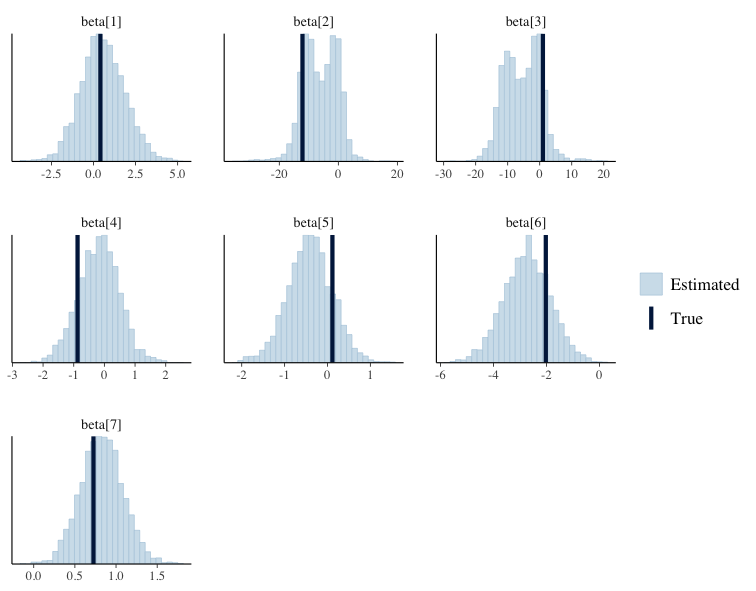
\includegraphics{./pic/Rplot01.png}

In the plot plot is the parameter recoverage of \(\phi\) parameters.
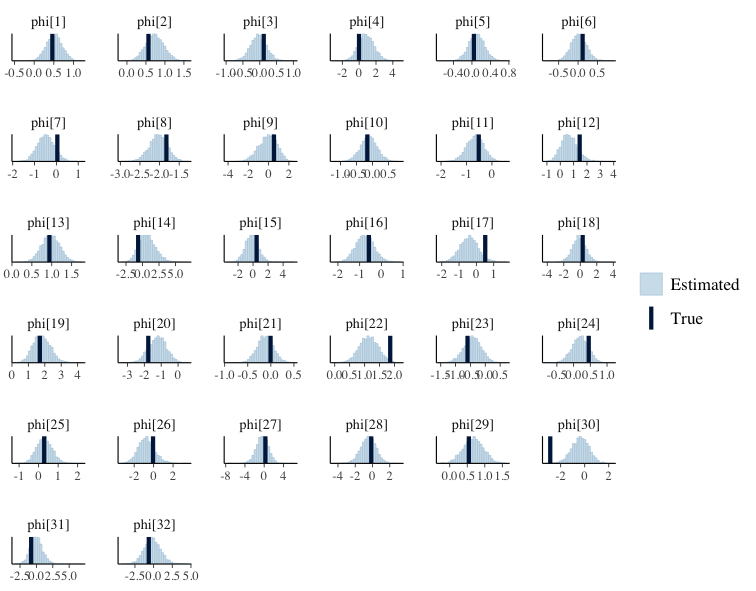
\includegraphics{./pic/Rplot.png} Finally, let's check the parameter
recoverage of \(\alpha,\theta,\tau\) 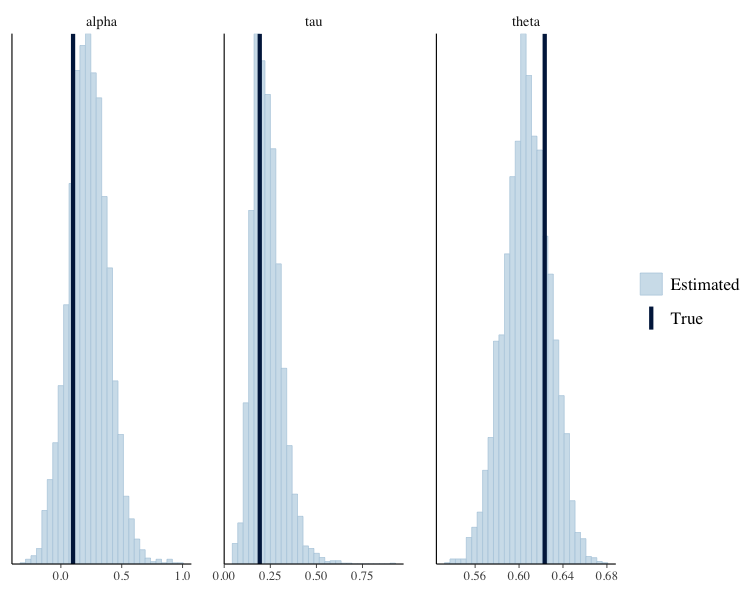
\includegraphics{./pic/Rplot02.png}

As we can see, all the parameters in our fake data recover very well.
This means it is reliable to use rstan to run this model.

\hypertarget{model-check}{%
\subsubsection{Model Check}\label{model-check}}

\hypertarget{posterior-predict-check-ppc}{%
\subparagraph{Posterior Predict Check
(PPC)}\label{posterior-predict-check-ppc}}

In the plot below we have the kernel density estimate of the observed
data (y, thicker curve) and 200 simulated data sets (\(y_{rep}\), thin
curves) from the posterior predictive distribution. If the model fits
the data well, as it does here, there is little difference between the
observed dataset and the simulated datasets.
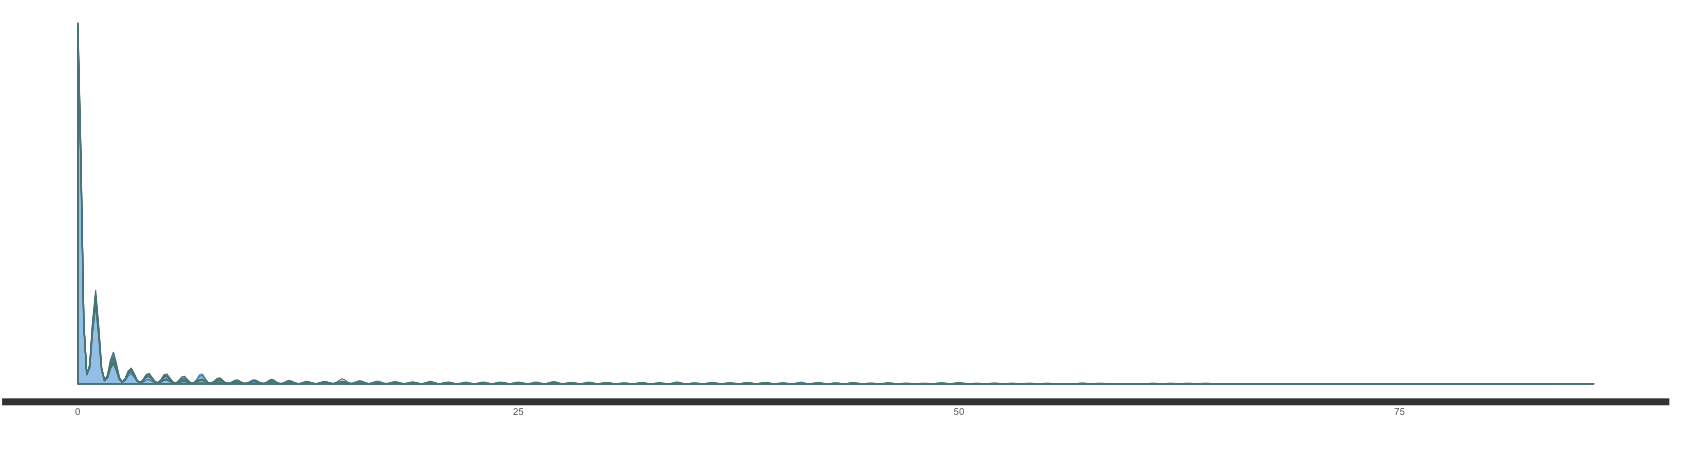
\includegraphics{./pic/Distributions-of-observed-data-and-a-random-sample-of-replications.png}

As we can see from the polt below, \(y_{rep}\) behavior well in the four
most common statistics. Ideally this vertical line would fall somewhere
within the histogram, as what we did.
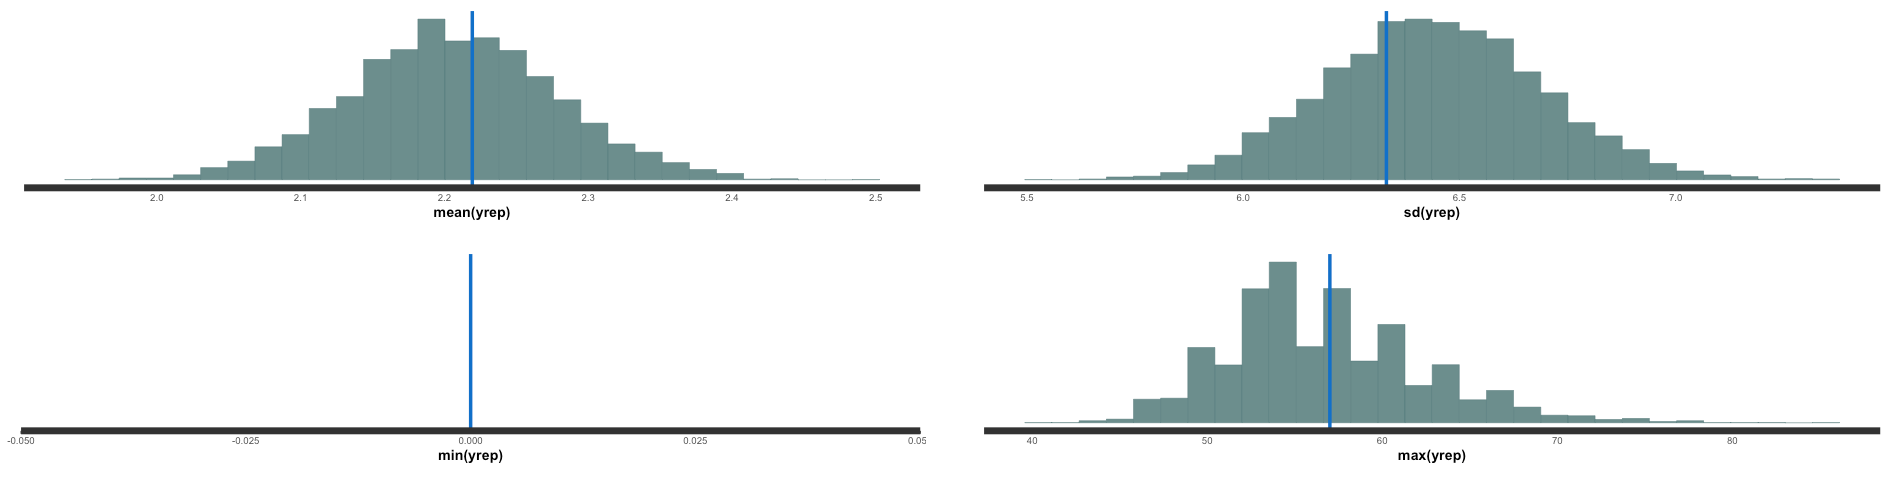
\includegraphics{./pic/Distributions-of-test-statistics.png .png}

The plot below shows the observed and average simulated value. As we can
see the model fit the data very well without obvious outliers.
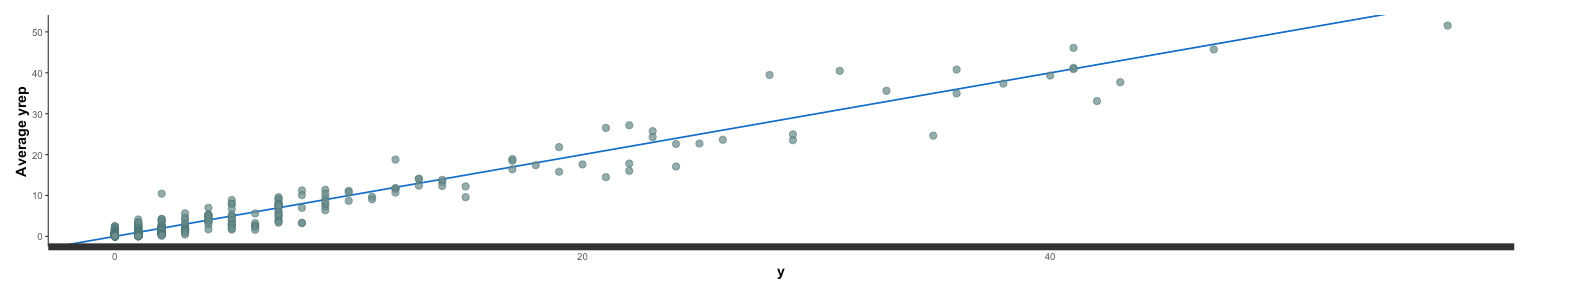
\includegraphics{./pic/observe-vs-average-simulated-value.png}

The residuals centered at 0 and have small variance. This indecates that
the model fit is acceptable.
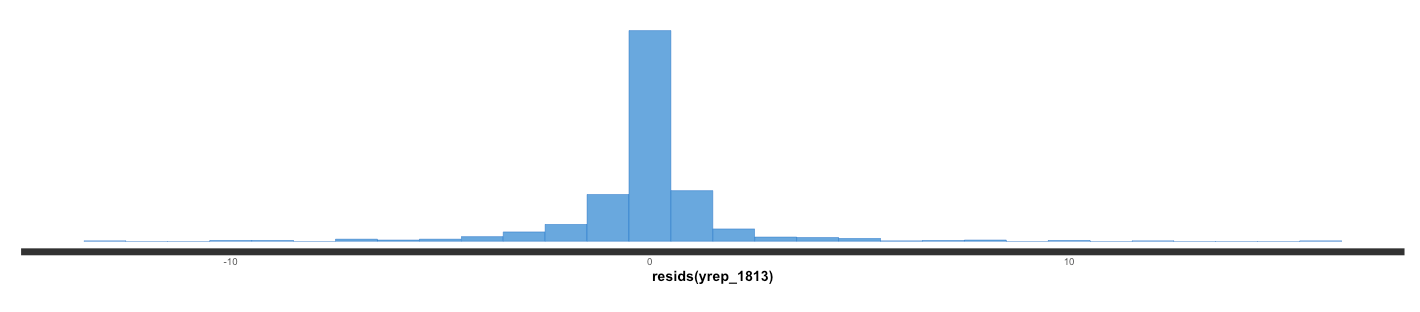
\includegraphics{./pic/residule-distribution.png}

\hypertarget{cross-validation-mse}{%
\subsubsection{Cross Validation \& MSE}\label{cross-validation-mse}}

In order to determine our model performance, again we do the 5-floder
cross validation. And we calculate the MSE for each training dataset
with our model. And then we get the average MSE. The stan code we used
to simulate the \(y_hat\) is as the following:

\begin{Shaded}
\begin{Highlighting}[]
\NormalTok{generated quantities\{}
\NormalTok{  int y_rep_cv[N_test];}
\NormalTok{  real}\OperatorTok{<}\NormalTok{lower =}\DecValTok{0}\NormalTok{,upper=}\DecValTok{1}\OperatorTok{>}\StringTok{ }\NormalTok{zero_test[N_test];}
  \ControlFlowTok{for}\NormalTok{ (i }\ControlFlowTok{in} \DecValTok{1}\OperatorTok{:}\NormalTok{N_test)\{}
\NormalTok{    zero_test[i] =}\StringTok{ }\KeywordTok{uniform_rng}\NormalTok{(}\DecValTok{0}\NormalTok{,}\DecValTok{1}\NormalTok{);}
    \ControlFlowTok{if}\NormalTok{ (zero_test[i] }\OperatorTok{<}\StringTok{ }\NormalTok{theta)\{}
\NormalTok{      y_rep_cv[i] =}\StringTok{ }\DecValTok{0}\NormalTok{;}
\NormalTok{      \}}
    \ControlFlowTok{else}\NormalTok{\{}
\NormalTok{      y_rep_cv[i] =}\StringTok{ }\KeywordTok{binomial_rng}\NormalTok{(n_city_test[i],}\KeywordTok{inv_logit}\NormalTok{( alpha[state_test[i]] }\OperatorTok{+}\StringTok{ }\NormalTok{X_test[i,]}\OperatorTok{*}\StringTok{ }\NormalTok{beta));}
\NormalTok{      \}}
\NormalTok{  \}}
\NormalTok{\}}
\end{Highlighting}
\end{Shaded}

Acrroding to the result, the baseline MSE is 128164. But for our model,
the average MSE is \textbf{7583} with the standard deviation
\textbf{6831}. Thus, we can say that our model have a huge improve from
the baseline.

\hypertarget{model-result}{%
\subsubsection{Model result}\label{model-result}}

\hypertarget{brief-results}{%
\paragraph{Brief results}\label{brief-results}}

In the following is the basic model results:

\begin{Shaded}
\begin{Highlighting}[]
\NormalTok{           mean se_mean   sd    }\FloatTok{2.5}\OperatorTok\StringTok{     }\DecValTok{50}\OperatorTok\StringTok{     }\DecValTok{98}\NormalTok{% n_eff Rhat}
\NormalTok{alpha     }\FloatTok{-2.67}    \FloatTok{0.00} \FloatTok{0.04}   \FloatTok{-2.76}   \FloatTok{-2.70}   \FloatTok{-2.67}   \FloatTok{-2.64}   \FloatTok{-2.59}   \DecValTok{187}  \FloatTok{1.0}
\NormalTok{beta[}\DecValTok{1}\NormalTok{]   }\FloatTok{-0.53}    \FloatTok{0.03} \FloatTok{0.38}   \FloatTok{-1.25}   \FloatTok{-0.80}   \FloatTok{-0.54}   \FloatTok{-0.29}    \FloatTok{0.25}   \DecValTok{143}  \FloatTok{1.0}
\NormalTok{beta[}\DecValTok{2}\NormalTok{]    }\FloatTok{0.19}    \FloatTok{0.23} \FloatTok{2.11}   \FloatTok{-4.74}   \FloatTok{-1.01}    \FloatTok{0.26}    \FloatTok{1.40}    \FloatTok{4.38}    \DecValTok{86}  \FloatTok{1.1}
\NormalTok{beta[}\DecValTok{3}\NormalTok{]    }\FloatTok{0.33}    \FloatTok{0.22} \FloatTok{2.09}   \FloatTok{-3.91}   \FloatTok{-0.84}    \FloatTok{0.26}    \FloatTok{1.48}    \FloatTok{5.04}    \DecValTok{94}  \FloatTok{1.0}
\NormalTok{beta[}\DecValTok{4}\NormalTok{]    }\FloatTok{0.32}    \FloatTok{0.03} \FloatTok{0.25}   \FloatTok{-0.18}    \FloatTok{0.16}    \FloatTok{0.32}    \FloatTok{0.50}    \FloatTok{0.83}    \DecValTok{97}  \FloatTok{1.1}
\NormalTok{beta[}\DecValTok{5}\NormalTok{]   }\FloatTok{-0.34}    \FloatTok{0.02} \FloatTok{0.20}   \FloatTok{-0.75}   \FloatTok{-0.48}   \FloatTok{-0.34}   \FloatTok{-0.21}    \FloatTok{0.06}   \DecValTok{109}  \FloatTok{1.1}
\NormalTok{beta[}\DecValTok{6}\NormalTok{]   }\FloatTok{-0.07}    \FloatTok{0.02} \FloatTok{0.21}   \FloatTok{-0.52}   \FloatTok{-0.21}   \FloatTok{-0.06}    \FloatTok{0.08}    \FloatTok{0.32}   \DecValTok{134}  \FloatTok{1.0}
\NormalTok{beta[}\DecValTok{7}\NormalTok{]   }\FloatTok{-0.18}    \FloatTok{0.01} \FloatTok{0.10}   \FloatTok{-0.36}   \FloatTok{-0.25}   \FloatTok{-0.18}   \FloatTok{-0.11}    \FloatTok{0.01}   \DecValTok{217}  \FloatTok{1.0}
\NormalTok{phi[}\DecValTok{1}\NormalTok{]    }\FloatTok{-0.09}    \FloatTok{0.00} \FloatTok{0.08}   \FloatTok{-0.24}   \FloatTok{-0.14}   \FloatTok{-0.09}   \FloatTok{-0.04}    \FloatTok{0.05}   \DecValTok{852}  \FloatTok{1.0}
\NormalTok{phi[}\DecValTok{2}\NormalTok{]     }\FloatTok{0.03}    \FloatTok{0.00} \FloatTok{0.08}   \FloatTok{-0.13}   \FloatTok{-0.02}    \FloatTok{0.03}    \FloatTok{0.08}    \FloatTok{0.19}  \DecValTok{2025}  \FloatTok{1.0}
\NormalTok{phi[}\DecValTok{3}\NormalTok{]    }\FloatTok{-0.23}    \FloatTok{0.00} \FloatTok{0.09}   \FloatTok{-0.41}   \FloatTok{-0.29}   \FloatTok{-0.22}   \FloatTok{-0.16}   \FloatTok{-0.05}  \DecValTok{1803}  \FloatTok{1.0}
\NormalTok{phi[}\DecValTok{4}\NormalTok{]     }\FloatTok{0.14}    \FloatTok{0.00} \FloatTok{0.12}   \FloatTok{-0.10}    \FloatTok{0.06}    \FloatTok{0.14}    \FloatTok{0.22}    \FloatTok{0.37}  \DecValTok{1829}  \FloatTok{1.0}
\NormalTok{phi[}\DecValTok{5}\NormalTok{]    }\FloatTok{-0.30}    \FloatTok{0.00} \FloatTok{0.11}   \FloatTok{-0.52}   \FloatTok{-0.37}   \FloatTok{-0.30}   \FloatTok{-0.23}   \FloatTok{-0.09}  \DecValTok{3299}  \FloatTok{1.0}
\NormalTok{phi[}\DecValTok{6}\NormalTok{]    }\FloatTok{-0.06}    \FloatTok{0.00} \FloatTok{0.10}   \FloatTok{-0.25}   \FloatTok{-0.12}   \FloatTok{-0.06}    \FloatTok{0.01}    \FloatTok{0.13}  \DecValTok{2359}  \FloatTok{1.0}
\NormalTok{phi[}\DecValTok{7}\NormalTok{]     }\FloatTok{0.09}    \FloatTok{0.00} \FloatTok{0.10}   \FloatTok{-0.11}    \FloatTok{0.02}    \FloatTok{0.09}    \FloatTok{0.15}    \FloatTok{0.28}  \DecValTok{2368}  \FloatTok{1.0}
\NormalTok{phi[}\DecValTok{8}\NormalTok{]     }\FloatTok{0.09}    \FloatTok{0.00} \FloatTok{0.10}   \FloatTok{-0.10}    \FloatTok{0.02}    \FloatTok{0.09}    \FloatTok{0.16}    \FloatTok{0.28}  \DecValTok{2423}  \FloatTok{1.0}
\NormalTok{phi[}\DecValTok{9}\NormalTok{]    }\FloatTok{-0.12}    \FloatTok{0.00} \FloatTok{0.12}   \FloatTok{-0.35}   \FloatTok{-0.20}   \FloatTok{-0.12}   \FloatTok{-0.04}    \FloatTok{0.12}  \DecValTok{3345}  \FloatTok{1.0}
\NormalTok{phi[}\DecValTok{10}\NormalTok{]    }\FloatTok{0.07}    \FloatTok{0.00} \FloatTok{0.11}   \FloatTok{-0.16}   \FloatTok{-0.01}    \FloatTok{0.07}    \FloatTok{0.14}    \FloatTok{0.28}  \DecValTok{2464}  \FloatTok{1.0}
\NormalTok{phi[}\DecValTok{11}\NormalTok{]   }\FloatTok{-0.10}    \FloatTok{0.00} \FloatTok{0.12}   \FloatTok{-0.35}   \FloatTok{-0.19}   \FloatTok{-0.10}   \FloatTok{-0.02}    \FloatTok{0.13}  \DecValTok{4003}  \FloatTok{1.0}
\NormalTok{phi[}\DecValTok{12}\NormalTok{]    }\FloatTok{0.16}    \FloatTok{0.00} \FloatTok{0.11}   \FloatTok{-0.06}    \FloatTok{0.08}    \FloatTok{0.16}    \FloatTok{0.23}    \FloatTok{0.36}  \DecValTok{2948}  \FloatTok{1.0}
\NormalTok{phi[}\DecValTok{13}\NormalTok{]   }\FloatTok{-0.45}    \FloatTok{0.00} \FloatTok{0.15}   \FloatTok{-0.76}   \FloatTok{-0.55}   \FloatTok{-0.44}   \FloatTok{-0.34}   \FloatTok{-0.15}  \DecValTok{3698}  \FloatTok{1.0}
\NormalTok{phi[}\DecValTok{14}\NormalTok{]    }\FloatTok{0.09}    \FloatTok{0.00} \FloatTok{0.13}   \FloatTok{-0.17}    \FloatTok{0.01}    \FloatTok{0.10}    \FloatTok{0.18}    \FloatTok{0.35}  \DecValTok{3833}  \FloatTok{1.0}
\NormalTok{phi[}\DecValTok{15}\NormalTok{]   }\FloatTok{-0.06}    \FloatTok{0.00} \FloatTok{0.14}   \FloatTok{-0.34}   \FloatTok{-0.15}   \FloatTok{-0.06}    \FloatTok{0.03}    \FloatTok{0.20}  \DecValTok{3366}  \FloatTok{1.0}
\NormalTok{phi[}\DecValTok{16}\NormalTok{]    }\FloatTok{0.28}    \FloatTok{0.00} \FloatTok{0.14}    \FloatTok{0.00}    \FloatTok{0.19}    \FloatTok{0.28}    \FloatTok{0.38}    \FloatTok{0.56}  \DecValTok{2951}  \FloatTok{1.0}
\NormalTok{phi[}\DecValTok{17}\NormalTok{]   }\FloatTok{-0.14}    \FloatTok{0.00} \FloatTok{0.16}   \FloatTok{-0.46}   \FloatTok{-0.25}   \FloatTok{-0.14}   \FloatTok{-0.03}    \FloatTok{0.15}  \DecValTok{4033}  \FloatTok{1.0}
\NormalTok{phi[}\DecValTok{18}\NormalTok{]   }\FloatTok{-0.45}    \FloatTok{0.00} \FloatTok{0.18}   \FloatTok{-0.80}   \FloatTok{-0.56}   \FloatTok{-0.45}   \FloatTok{-0.33}   \FloatTok{-0.12}  \DecValTok{1581}  \FloatTok{1.0}
\NormalTok{phi[}\DecValTok{19}\NormalTok{]    }\FloatTok{0.08}    \FloatTok{0.00} \FloatTok{0.16}   \FloatTok{-0.24}   \FloatTok{-0.03}    \FloatTok{0.08}    \FloatTok{0.19}    \FloatTok{0.39}  \DecValTok{4147}  \FloatTok{1.0}
\NormalTok{phi[}\DecValTok{20}\NormalTok{]    }\FloatTok{0.40}    \FloatTok{0.00} \FloatTok{0.16}    \FloatTok{0.10}    \FloatTok{0.29}    \FloatTok{0.40}    \FloatTok{0.51}    \FloatTok{0.70}  \DecValTok{1102}  \FloatTok{1.0}
\NormalTok{phi[}\DecValTok{21}\NormalTok{]   }\FloatTok{-0.08}    \FloatTok{0.00} \FloatTok{0.17}   \FloatTok{-0.41}   \FloatTok{-0.20}   \FloatTok{-0.08}    \FloatTok{0.04}    \FloatTok{0.25}  \DecValTok{4140}  \FloatTok{1.0}
\NormalTok{phi[}\DecValTok{22}\NormalTok{]    }\FloatTok{0.04}    \FloatTok{0.00} \FloatTok{0.18}   \FloatTok{-0.31}   \FloatTok{-0.08}    \FloatTok{0.04}    \FloatTok{0.16}    \FloatTok{0.37}  \DecValTok{4044}  \FloatTok{1.0}
\NormalTok{phi[}\DecValTok{23}\NormalTok{]    }\FloatTok{0.22}    \FloatTok{0.00} \FloatTok{0.18}   \FloatTok{-0.13}    \FloatTok{0.10}    \FloatTok{0.22}    \FloatTok{0.34}    \FloatTok{0.56}  \DecValTok{2248}  \FloatTok{1.0}
\NormalTok{phi[}\DecValTok{24}\NormalTok{]    }\FloatTok{0.33}    \FloatTok{0.00} \FloatTok{0.18}   \FloatTok{-0.03}    \FloatTok{0.21}    \FloatTok{0.33}    \FloatTok{0.45}    \FloatTok{0.69}  \DecValTok{3626}  \FloatTok{1.0}
\NormalTok{phi[}\DecValTok{25}\NormalTok{]    }\FloatTok{0.10}    \FloatTok{0.00} \FloatTok{0.20}   \FloatTok{-0.30}   \FloatTok{-0.03}    \FloatTok{0.10}    \FloatTok{0.23}    \FloatTok{0.47}  \DecValTok{3735}  \FloatTok{1.0}
\NormalTok{phi[}\DecValTok{26}\NormalTok{]   }\FloatTok{-0.05}    \FloatTok{0.00} \FloatTok{0.23}   \FloatTok{-0.53}   \FloatTok{-0.20}   \FloatTok{-0.05}    \FloatTok{0.11}    \FloatTok{0.38}  \DecValTok{3186}  \FloatTok{1.0}
\NormalTok{phi[}\DecValTok{27}\NormalTok{]    }\FloatTok{0.23}    \FloatTok{0.00} \FloatTok{0.20}   \FloatTok{-0.16}    \FloatTok{0.10}    \FloatTok{0.23}    \FloatTok{0.37}    \FloatTok{0.63}  \DecValTok{2633}  \FloatTok{1.0}
\NormalTok{phi[}\DecValTok{28}\NormalTok{]    }\FloatTok{0.01}    \FloatTok{0.00} \FloatTok{0.20}   \FloatTok{-0.39}   \FloatTok{-0.11}    \FloatTok{0.01}    \FloatTok{0.15}    \FloatTok{0.38}  \DecValTok{3371}  \FloatTok{1.0}
\NormalTok{phi[}\DecValTok{29}\NormalTok{]   }\FloatTok{-0.26}    \FloatTok{0.00} \FloatTok{0.23}   \FloatTok{-0.73}   \FloatTok{-0.41}   \FloatTok{-0.25}   \FloatTok{-0.10}    \FloatTok{0.18}  \DecValTok{2812}  \FloatTok{1.0}
\NormalTok{phi[}\DecValTok{30}\NormalTok{]   }\FloatTok{-0.29}    \FloatTok{0.00} \FloatTok{0.20}   \FloatTok{-0.70}   \FloatTok{-0.41}   \FloatTok{-0.28}   \FloatTok{-0.15}    \FloatTok{0.07}  \DecValTok{1902}  \FloatTok{1.0}
\NormalTok{phi[}\DecValTok{31}\NormalTok{]   }\FloatTok{-0.03}    \FloatTok{0.00} \FloatTok{0.25}   \FloatTok{-0.55}   \FloatTok{-0.19}   \FloatTok{-0.02}    \FloatTok{0.14}    \FloatTok{0.44}  \DecValTok{3394}  \FloatTok{1.0}
\NormalTok{phi[}\DecValTok{32}\NormalTok{]    }\FloatTok{0.35}    \FloatTok{0.00} \FloatTok{0.26}   \FloatTok{-0.16}    \FloatTok{0.18}    \FloatTok{0.35}    \FloatTok{0.53}    \FloatTok{0.86}  \DecValTok{3258}  \FloatTok{1.0}
\NormalTok{theta      }\FloatTok{0.01}    \FloatTok{0.00} \FloatTok{0.01}    \FloatTok{0.00}    \FloatTok{0.00}    \FloatTok{0.01}    \FloatTok{0.01}    \FloatTok{0.03}   \DecValTok{213}  \FloatTok{1.0}
\NormalTok{tau        }\FloatTok{2.49}    \FloatTok{0.05} \FloatTok{0.84}    \FloatTok{1.23}    \FloatTok{1.88}    \FloatTok{2.37}    \FloatTok{2.98}    \FloatTok{4.46}   \DecValTok{240}  \FloatTok{1.0}
\NormalTok{lp__    }\FloatTok{-812.85}    \FloatTok{0.20} \FloatTok{4.82} \FloatTok{-823.32} \FloatTok{-815.77} \FloatTok{-812.58} \FloatTok{-809.53} \FloatTok{-804.33}   \DecValTok{593}  \FloatTok{1.0}
\end{Highlighting}
\end{Shaded}

A quick check for the Rhat in our model is all very good. The posterior
confidence interval of the parameters are show as the following plots.

\hypertarget{confidence-intervial-and-interpretation}{%
\paragraph{Confidence intervial and
interpretation}\label{confidence-intervial-and-interpretation}}

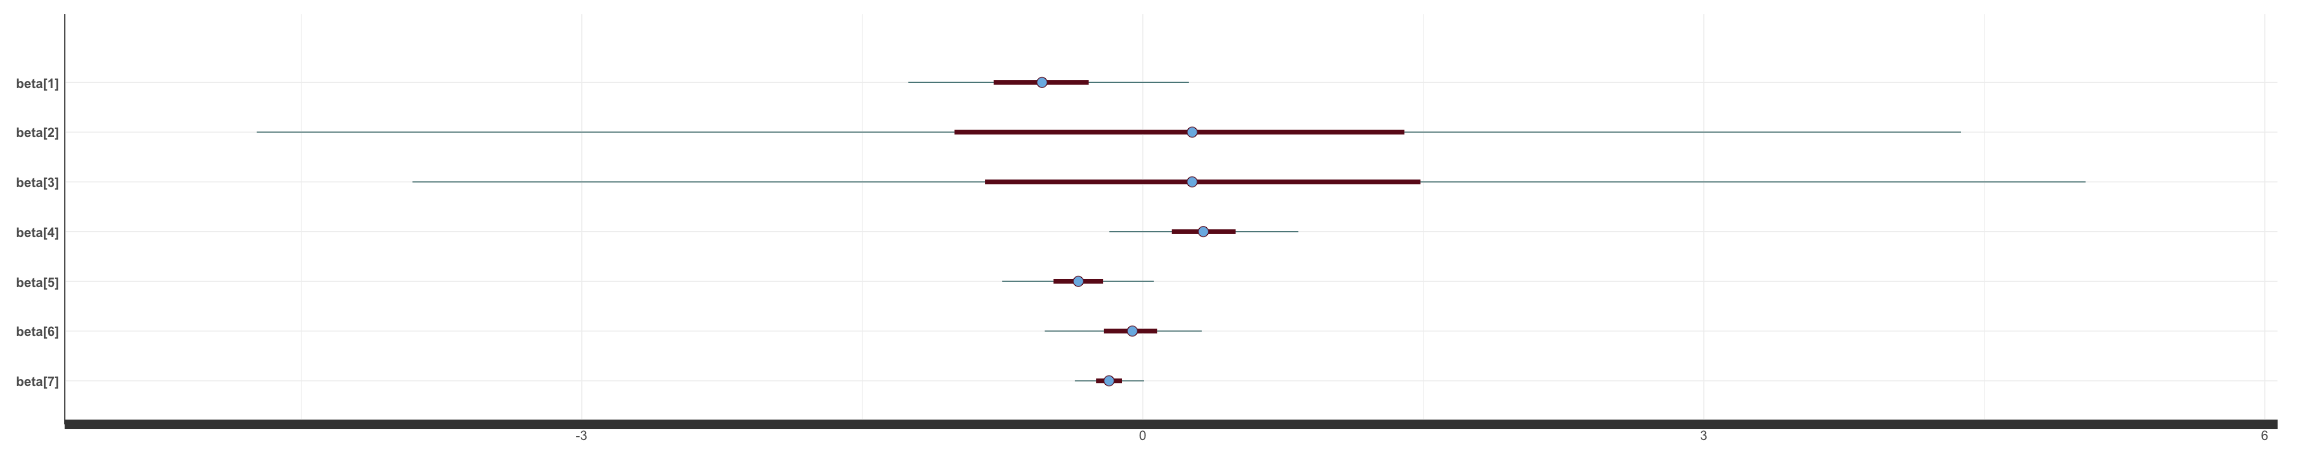
\includegraphics{./pic/posterior-distribution-of-betas.png}

As we can see above, the effect from the age is significant based on the
95\% confidence interval. Other parameter are not significant enough.

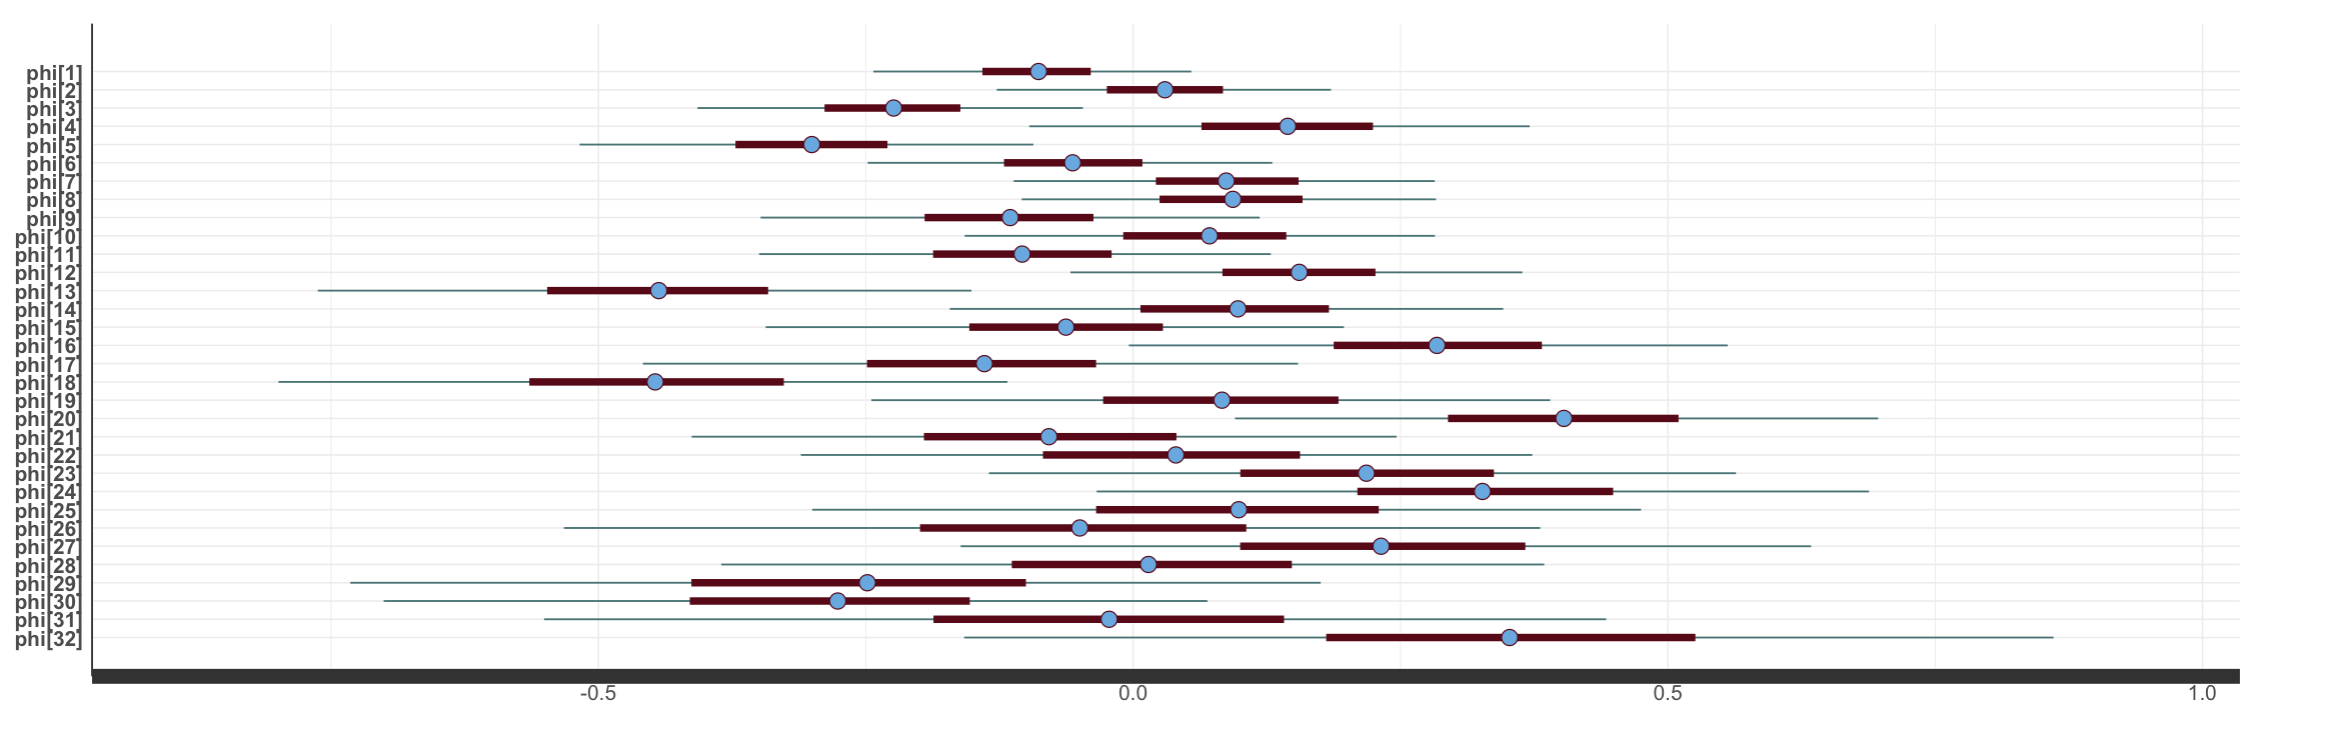
\includegraphics{./pic/posterior-distribution-of-state-effects.png}

The state effects are obvious. We can see that \(\phi_3\) (QUERETARO DE
ARTEAGA), \(\phi_5\) (GUANAJUATO) , \(\phi_{13}\) (AGUASCALIENTES) and
\(\phi_{18}\) (VERACRUZ LLAVE) have the nigative effect, which means
these state is less likely to have default. However, \(\phi_{20}\)
(MICHOACAN DE OCAMPO) has a significantly postive effect.

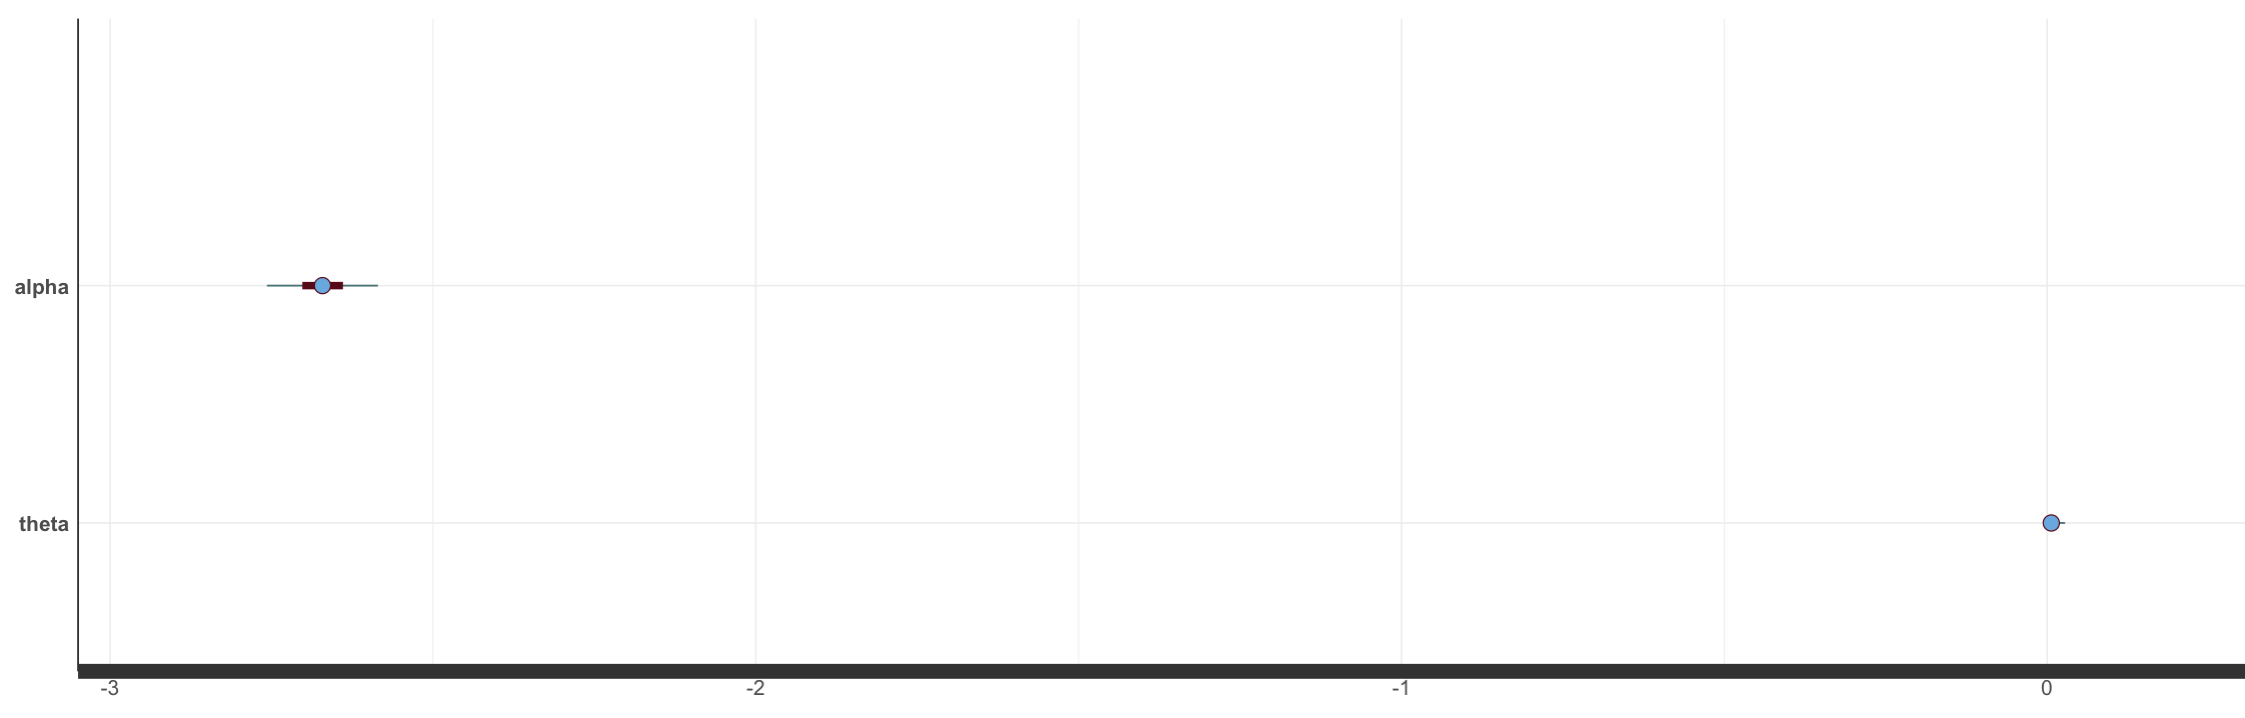
\includegraphics{./pic/posterior-distribution-of-theta-alpha.png} As we
can see, the overall offset effect is obvious that for about -2.67. And
on avrage, there will have 1\% of cities have no default at all. On 95\%
confidence interval, there will have less than 3\% of cities have no
default.

\hypertarget{conclusion}{%
\section{Conclusion}\label{conclusion}}

\hypertarget{exercises-and-extensions}{%
\section{Exercises and Extensions}\label{exercises-and-extensions}}

\hypertarget{model-discussion-individual-level-analysis}{%
\subsection{Model discussion: Individual level
Analysis}\label{model-discussion-individual-level-analysis}}

In the past chapters, we focus on the city level analysis. In this way,
we simplified our data set and clearified our model design ideas. More
importantly, it saves a lot of time to run this model in city level.
However, in reality, people may also interested in the individual
default risk. Besides, some independent variables like average age is
not make so much sense.

In this chapter, we will instead run the model for the individual level.
For individual level, it's more resonable to use the logistic regression
instead of the binormial regression. \[p(y_i) =\begin{cases} 
1, & defaule \space at \space least \space once \\
0, & otherwise \end{cases}\] However, the CAR still can be used.Thus,
the new model for individual level can be summarized as these:
\[ y_{ij} \sim bernoulli(logit^{-1}(a + \phi_j + x_{ij}\beta)) \] As the
same the zero-inflated model extension will also be applied in the
individual level. \[p(y_i | \theta,a,\beta) =\begin{cases}  
\theta + (1-\theta) \times bernoulli(0 |a,\beta,\phi ) & y_i =0 \\
(1-\theta) \times bernoulli(0 |a,\beta,\phi )  & y_i > 0 \end{cases}\]

The model result is in the following:

\begin{Shaded}
\begin{Highlighting}[]
\NormalTok{            mean se_mean    sd       }\DecValTok{1}\NormalTok{% n_eff Rhat}
\NormalTok{alpha      }\FloatTok{-0.82}    \FloatTok{0.18}  \FloatTok{1.09}    \FloatTok{-2.64}    \DecValTok{36} \FloatTok{1.11}
\NormalTok{beta[}\DecValTok{1}\NormalTok{]    }\FloatTok{-0.13}    \FloatTok{0.02}  \FloatTok{0.18}    \FloatTok{-0.56}   \DecValTok{100} \FloatTok{1.04}
\NormalTok{beta[}\DecValTok{2}\NormalTok{]     }\FloatTok{0.08}    \FloatTok{0.04}  \FloatTok{0.25}    \FloatTok{-0.26}    \DecValTok{32} \FloatTok{1.13}
\NormalTok{beta[}\DecValTok{3}\NormalTok{]     }\FloatTok{0.03}    \FloatTok{0.06}  \FloatTok{0.27}    \FloatTok{-1.08}    \DecValTok{23} \FloatTok{1.14}
\NormalTok{beta[}\DecValTok{4}\NormalTok{]     }\FloatTok{0.01}    \FloatTok{0.03}  \FloatTok{0.15}    \FloatTok{-0.29}    \DecValTok{27} \FloatTok{1.14}
\NormalTok{beta[}\DecValTok{5}\NormalTok{]    }\FloatTok{-0.08}    \FloatTok{0.05}  \FloatTok{0.27}    \FloatTok{-0.67}    \DecValTok{30} \FloatTok{1.13}
\NormalTok{beta[}\DecValTok{6}\NormalTok{]    }\FloatTok{-0.27}    \FloatTok{0.04}  \FloatTok{0.23}    \FloatTok{-1.03}    \DecValTok{30} \FloatTok{1.13}
\NormalTok{beta[}\DecValTok{7}\NormalTok{]    }\FloatTok{-0.02}    \FloatTok{0.00}  \FloatTok{0.06}    \FloatTok{-0.22}   \DecValTok{154} \FloatTok{1.01}
\NormalTok{phi[}\DecValTok{1}\NormalTok{]     }\FloatTok{-0.11}    \FloatTok{0.01}  \FloatTok{0.29}    \FloatTok{-0.85}  \DecValTok{3132} \FloatTok{1.00}
\NormalTok{phi[}\DecValTok{2}\NormalTok{]      }\FloatTok{0.16}    \FloatTok{0.00}  \FloatTok{0.25}    \FloatTok{-0.45}  \DecValTok{3095} \FloatTok{1.00}
\NormalTok{phi[}\DecValTok{3}\NormalTok{]     }\FloatTok{-0.14}    \FloatTok{0.01}  \FloatTok{0.14}    \FloatTok{-0.60}   \DecValTok{101} \FloatTok{1.04}
\NormalTok{phi[}\DecValTok{4}\NormalTok{]      }\FloatTok{0.27}    \FloatTok{0.01}  \FloatTok{0.34}    \FloatTok{-0.43}   \DecValTok{543} \FloatTok{1.01}
\NormalTok{phi[}\DecValTok{5}\NormalTok{]      }\FloatTok{0.02}    \FloatTok{0.00}  \FloatTok{0.24}    \FloatTok{-0.58}  \DecValTok{3944} \FloatTok{1.00}
\NormalTok{phi[}\DecValTok{6}\NormalTok{]      }\FloatTok{0.36}    \FloatTok{0.03}  \FloatTok{0.30}    \FloatTok{-0.10}   \DecValTok{110} \FloatTok{1.03}
\NormalTok{phi[}\DecValTok{7}\NormalTok{]      }\FloatTok{0.04}    \FloatTok{0.00}  \FloatTok{0.15}    \FloatTok{-0.30}  \DecValTok{3151} \FloatTok{1.00}
\NormalTok{phi[}\DecValTok{8}\NormalTok{]     }\FloatTok{-0.41}    \FloatTok{0.03}  \FloatTok{0.22}    \FloatTok{-1.18}    \DecValTok{43} \FloatTok{1.09}
\NormalTok{phi[}\DecValTok{9}\NormalTok{]     }\FloatTok{-0.15}    \FloatTok{0.01}  \FloatTok{0.22}    \FloatTok{-0.82}   \DecValTok{637} \FloatTok{1.01}
\NormalTok{phi[}\DecValTok{10}\NormalTok{]    }\FloatTok{-0.69}    \FloatTok{0.04}  \FloatTok{0.34}    \FloatTok{-1.82}    \DecValTok{81} \FloatTok{1.05}
\NormalTok{phi[}\DecValTok{11}\NormalTok{]     }\FloatTok{0.17}    \FloatTok{0.00}  \FloatTok{0.18}    \FloatTok{-0.21}  \DecValTok{1320} \FloatTok{1.01}
\NormalTok{phi[}\DecValTok{12}\NormalTok{]     }\FloatTok{0.15}    \FloatTok{0.01}  \FloatTok{0.20}    \FloatTok{-0.25}   \DecValTok{537} \FloatTok{1.01}
\NormalTok{phi[}\DecValTok{13}\NormalTok{]     }\FloatTok{0.82}    \FloatTok{0.04}  \FloatTok{0.36}     \FloatTok{0.24}    \DecValTok{84} \FloatTok{1.05}
\NormalTok{phi[}\DecValTok{14}\NormalTok{]     }\FloatTok{0.55}    \FloatTok{0.03}  \FloatTok{0.38}    \FloatTok{-0.10}   \DecValTok{123} \FloatTok{1.04}
\NormalTok{phi[}\DecValTok{15}\NormalTok{]     }\FloatTok{0.19}    \FloatTok{0.01}  \FloatTok{0.17}    \FloatTok{-0.16}   \DecValTok{655} \FloatTok{1.01}
\NormalTok{phi[}\DecValTok{16}\NormalTok{]    }\FloatTok{-0.48}    \FloatTok{0.03}  \FloatTok{0.24}    \FloatTok{-1.25}    \DecValTok{53} \FloatTok{1.07}
\NormalTok{phi[}\DecValTok{17}\NormalTok{]    }\FloatTok{-0.41}    \FloatTok{0.02}  \FloatTok{0.25}    \FloatTok{-1.23}   \DecValTok{117} \FloatTok{1.03}
\NormalTok{phi[}\DecValTok{18}\NormalTok{]    }\FloatTok{-0.11}    \FloatTok{0.01}  \FloatTok{0.16}    \FloatTok{-0.59}   \DecValTok{664} \FloatTok{1.01}
\NormalTok{phi[}\DecValTok{19}\NormalTok{]    }\FloatTok{-0.20}    \FloatTok{0.01}  \FloatTok{0.24}    \FloatTok{-0.91}   \DecValTok{682} \FloatTok{1.01}
\NormalTok{phi[}\DecValTok{20}\NormalTok{]     }\FloatTok{0.47}    \FloatTok{0.04}  \FloatTok{0.36}    \FloatTok{-0.08}    \DecValTok{89} \FloatTok{1.04}
\NormalTok{phi[}\DecValTok{21}\NormalTok{]    }\FloatTok{-0.17}    \FloatTok{0.01}  \FloatTok{0.21}    \FloatTok{-0.82}   \DecValTok{466} \FloatTok{1.01}
\NormalTok{phi[}\DecValTok{22}\NormalTok{]    }\FloatTok{-0.13}    \FloatTok{0.00}  \FloatTok{0.22}    \FloatTok{-0.73}  \DecValTok{2394} \FloatTok{1.00}
\NormalTok{phi[}\DecValTok{23}\NormalTok{]     }\FloatTok{0.07}    \FloatTok{0.00}  \FloatTok{0.21}    \FloatTok{-0.45}  \DecValTok{3670} \FloatTok{1.00}
\NormalTok{phi[}\DecValTok{24}\NormalTok{]    }\FloatTok{-0.03}    \FloatTok{0.01}  \FloatTok{0.33}    \FloatTok{-0.79}  \DecValTok{3470} \FloatTok{1.00}
\NormalTok{phi[}\DecValTok{25}\NormalTok{]     }\FloatTok{0.07}    \FloatTok{0.01}  \FloatTok{0.29}    \FloatTok{-0.59}  \DecValTok{1547} \FloatTok{1.01}
\NormalTok{phi[}\DecValTok{26}\NormalTok{]     }\FloatTok{0.23}    \FloatTok{0.02}  \FloatTok{0.28}    \FloatTok{-0.26}   \DecValTok{163} \FloatTok{1.03}
\NormalTok{phi[}\DecValTok{27}\NormalTok{]     }\FloatTok{0.65}    \FloatTok{0.03}  \FloatTok{0.38}     \FloatTok{0.04}   \DecValTok{135} \FloatTok{1.03}
\NormalTok{phi[}\DecValTok{28}\NormalTok{]    }\FloatTok{-0.74}    \FloatTok{0.04}  \FloatTok{0.48}    \FloatTok{-2.24}   \DecValTok{180} \FloatTok{1.03}
\NormalTok{phi[}\DecValTok{29}\NormalTok{]     }\FloatTok{0.10}    \FloatTok{0.01}  \FloatTok{0.33}    \FloatTok{-0.71}  \DecValTok{3152} \FloatTok{1.00}
\NormalTok{phi[}\DecValTok{30}\NormalTok{]    }\FloatTok{-0.35}    \FloatTok{0.01}  \FloatTok{0.31}    \FloatTok{-1.24}   \DecValTok{762} \FloatTok{1.01}
\NormalTok{phi[}\DecValTok{31}\NormalTok{]    }\FloatTok{-0.15}    \FloatTok{0.01}  \FloatTok{0.34}    \FloatTok{-1.05}  \DecValTok{2137} \FloatTok{1.00}
\NormalTok{phi[}\DecValTok{32}\NormalTok{]    }\FloatTok{-0.02}    \FloatTok{0.01}  \FloatTok{0.37}    \FloatTok{-0.99}  \DecValTok{3879} \FloatTok{1.00}
\NormalTok{theta       }\FloatTok{0.69}    \FloatTok{0.03}  \FloatTok{0.23}     \FloatTok{0.05}    \DecValTok{64} \FloatTok{1.06}
\NormalTok{lp__    }\FloatTok{-7215.11}    \FloatTok{2.34} \FloatTok{13.51} \FloatTok{-7251.54}    \DecValTok{33} \FloatTok{1.11}
\end{Highlighting}
\end{Shaded}

Clearly, the individual level model did not converge as well as the city
level model. And it takes much more time. But We can still get lots of
useful information from the result:

\begin{enumerate}
\def\labelenumi{\arabic{enumi}.}
\item
  About 69\% of the invdividual would not defalut at all.
\item
  Compared with the city level model, the independent variables' effects
  and state effects tends to be more obvious with smaller standard
  deviation. And the result is consistant.
\end{enumerate}

\hypertarget{other-discussion}{%
\subsection{Other Discussion}\label{other-discussion}}

This case study's idea can be easily applied and extended for realistic
applications in several obvious ways. Just like we did in the individual
level analysis. There are some other thinking about this case study.

\begin{enumerate}
\def\labelenumi{\arabic{enumi}.}
\item
  \emph{Simulation-based calibration}. Write a Stan model to simulate
  data from this model. First simulate parameters from the prior (or
  pick ones consistent with the priors). Then simulate data from the
  parameters. Finally, fit the model in Stan and compare the coverage as
  in the last plot in the case study.
\item
  \emph{Forecasting and backcasting}. Extend predictions another 50
  years into the future and plot as in the last plot. This can be done
  by extending the solution points in the transformed parameters, but is
  more efficiently done in the generated quantities block. Next, extend
  the predictions 50 years into the past and plot.
\item
  \emph{Missing data}. Suppose that several of the measurements are
  missing. Write a Stan program that uses only the observed
  measurements. This will require coding the data in long form. Only
  this part of the model changes; the ODE is set up and fit as before
  with the complete set of time points. What happens to the computation
  and posterior inferences as increasing amounts of data are missing?
  How can the missing data points be imputed using the generated
  quantities block?38
\item
  \emph{Error model}. Replace the lognormal error with a simple normal
  error model. What does this do to the z estimates and to the basic
  parameter estimates? Which error model fits better?
\item
  \emph{Sensitivity analysis and prior choice}. Perform a sensitivity
  analysis on the prior choices made for this model. When the prior
  means or scales are varied, how much does the posterior vary? Does the
  model become easier or harder to fit (in terms of effective sample
  size per unit time or divergent transitions) with different prior
  choices? What does this imply about the number of digits with which we
  report results and thus the effective sample sizes necessary for most
  inferences?
\item
  \emph{Model misspecification}. Swap the coding of the lynx and hare in
  the input so that the predator is modeled as prey and vice-versa. How
  well does it fit the data? How does this provide evidence for the folk
  theorem?
\end{enumerate}

\hypertarget{references}{%
\subsection*{References}\label{references}}
\addcontentsline{toc}{subsection}{References}

\begin{itemize}
\tightlist
\item
  Besag, Julian, Jeremy York, and Annie Mollié. (1991) Bayesian image
  restoration, with two applications in spatial statistics. \emph{Annals
  of the institute of statistical mathematics}, 43.1: 1-20.
\item
  Gelfand, Alan E., and Penelope Vounatsou. (2003) Proper multivariate
  conditional autoregressive models for spatial data analysis.
  \emph{Biostatistics} 4.1: 11-15.
\item
  Jin, Xiaoping, Bradley P. Carlin, and Sudipto Banerjee. (2005)
  Generalized hierarchical multivariate CAR models for areal data.
  \emph{Biometrics} 61.4: 950-961.
\item
  Bob Carpenter. (2018)
  \href{http://mc-stan.org/users/documentation/case-studies/lotka-volterra-predator-prey.html\#data-lynx-and-hare-pelts-in-canada}{Predator-Prey
  Population Dynamics: the Lotka-Volterra model in Stan}. \emph{Rstan
  Document For Example}.
\item
  Max Joseph. (2011)
  \href{http://mc-stan.org/users/documentation/case-studies/mbjoseph-CARStan.html}{Exact
  sparse CAR models in Stan}. \emph{Rstan Document For Example}.
\item
  Stan Development Team (2017) \emph{Stan Modeling Language Users Guide
  and Reference Manual}, Version 2.17, \url{http://mc-stan.org}.
\item
  Vehtari, A., Gelman, A. \& Gabry, J. (2017) Practical Bayesian model
  evaluation using leave-one-out cross-validation and WAIC.
  \emph{Journal of Statistics and Computing} 27(5):1413--1432.
\item
  Andrew Gelman, John B. Carlin, Hal S. Stern, David B. Dunson, Aki
  Vehtari, Donald B. Rubin (2014)
  \href{https://www.google.com/search?q=bayesian+data+analysis\&oq=bayesian+data+analysis\&aqs=chrome.0.69i59j69i60l2j69i61j69i65j0.3253j1j4\&sourceid=chrome\&ie=UTF-8}{\emph{Bayesian
  Data Analysis}}
\item
  Stan Development Team (2018)
  \href{http://www.stat.columbia.edu/~gelman/bda.course/_book/}{\emph{Bayesian
  Statistics Using Stan}}
\end{itemize}

\hypertarget{source-code}{%
\subsection*{Source code}\label{source-code}}
\addcontentsline{toc}{subsection}{Source code}

All of the source code, data, text, and images for this case study are
available on GitHub at: *
\href{https://github.com/ChrisChen0429/BDA_project}{A bayesian approach
to indentify morgage default rate at city level}

\hypertarget{complete-stan-program}{%
\subsection*{Complete Stan program}\label{complete-stan-program}}
\addcontentsline{toc}{subsection}{Complete Stan program}

The complete Stn program for this case study are available on the google
at: *
\href{https://docs.google.com/document/d/1N0XtUlnsnYi_bInkrbTQG2DCD1Hf7mXaSoZWQbWrOqg/edit?usp=sharing}{A
bayesian approach to indentify morgage default rate at city level}

\hypertarget{acknowledgements}{%
\subsection*{Acknowledgements}\label{acknowledgements}}
\addcontentsline{toc}{subsection}{Acknowledgements}

Thanks to Simon Woodward, Arya Pourzanjani, and Leo Lahti for helpful
comments on earlier drafts and Peter Howard for providing the provenance
of the data and the original case study with the data.

\hypertarget{session-information}{%
\subsection*{Session information}\label{session-information}}
\addcontentsline{toc}{subsection}{Session information}

\begin{Shaded}
\begin{Highlighting}[]
\KeywordTok{sessionInfo}\NormalTok{()}
\end{Highlighting}
\end{Shaded}

\begin{verbatim}
R version 3.5.1 (2018-07-02)
Platform: x86_64-apple-darwin17.6.0 (64-bit)
Running under: macOS  10.14.1

Matrix products: default
BLAS: /System/Library/Frameworks/Accelerate.framework/Versions/A/Frameworks/vecLib.framework/Versions/A/libBLAS.dylib
LAPACK: /System/Library/Frameworks/Accelerate.framework/Versions/A/Frameworks/vecLib.framework/Versions/A/libLAPACK.dylib

locale:
[1] en_US.UTF-8/en_US.UTF-8/en_US.UTF-8/C/en_US.UTF-8/en_US.UTF-8

attached base packages:
[1] stats     graphics  grDevices utils    
[5] datasets  methods   base     

other attached packages:
[1] tufte_0.4          rstan_2.18.2      
[3] StanHeaders_2.18.0 reshape_0.8.8     
[5] knitr_1.20         gridExtra_2.3     
[7] ggplot2_3.1.0     

loaded via a namespace (and not attached):
 [1] Rcpp_1.0.0         formatR_1.5       
 [3] pillar_1.3.0       compiler_3.5.1    
 [5] plyr_1.8.4         bindr_0.1.1       
 [7] prettyunits_1.0.2  base64enc_0.1-3   
 [9] tools_3.5.1        pkgbuild_1.0.2    
[11] digest_0.6.18      evaluate_0.12     
[13] tibble_1.4.2       gtable_0.2.0      
[15] pkgconfig_2.0.2    rlang_0.3.0.1     
[17] cli_1.0.1          parallel_3.5.1    
[19] yaml_2.2.0         loo_2.0.0.9000    
[21] bindrcpp_0.2.2     withr_2.1.2       
[23] dplyr_0.7.8        stringr_1.3.1     
[25] stats4_3.5.1       rprojroot_1.3-2   
[27] grid_3.5.1         tidyselect_0.2.5  
[29] inline_0.3.15      glue_1.3.0        
[31] R6_2.3.0           processx_3.2.0    
[33] rmarkdown_1.10     callr_3.0.0       
[35] purrr_0.2.5        magrittr_1.5      
[37] matrixStats_0.54.0 ps_1.2.1          
[39] backports_1.1.2    scales_1.0.0      
[41] htmltools_0.3.6    assertthat_0.2.0  
[43] colorspace_1.3-2   stringi_1.2.4     
[45] lazyeval_0.2.1     munsell_0.5.0     
[47] crayon_1.3.4      
\end{verbatim}

\hypertarget{licenses}{%
\subsection*{Licenses}\label{licenses}}
\addcontentsline{toc}{subsection}{Licenses}

{Code © 2017--2018, Columbia University in New York, licensed under
BSD-3.}

{Text © Andres Potapczynski, Jongwoo Choi, Yi Chen }



\end{document}
